%!TEX program = xelatex
% !BIB program = bibtex
\documentclass[12pt,letterpaper]{article}
\usepackage{./style/dsc180reportstyle} % import dsc180reportstyle.sty

%%%%%%%%%%%%%%%%%%%%%%%%%%%%%%%%%%%%%%%%%%%%%%%%%%%%%%%%
%%%% Title and Authors
%%%%%%%%%%%%%%%%%%%%%%%%%%%%%%%%%%%%%%%%%%%%%%%%%%%%%%%%

\title{Novel Techniques in Private Telemetry Analysis}

\author{Trey Scheid \\
  {\tt tscheid@ucsd.edu} \\\And
  Tyler Kurpanek \\
  {\tt tkurpane@ucsd.edu} \\\And
  Bradley Nathanson \\
  {\tt bnathanson@ucsd.edu} \\\And
  Christopher Lum \\
  {\tt cslum@ucsd.edu} \\\And
  Yu-Xiang Wang \\
  {\tt yuxiangw@ucsd.edu} \\}

\begin{document}
% INSERT TITLE
% title is defined above
\maketitle



%%%%%%%%%%%%%%%%%%%%%%%%%%%%%%%%%%%%%%%%%%%%%%%%%%%%%%%%
%%%% Abstract and Links
%%%%%%%%%%%%%%%%%%%%%%%%%%%%%%%%%%%%%%%%%%%%%%%%%%%%%%%%

\begin{abstract}    
  \textcolor{LightGrey}{Is the abstract supposed to be in light gray as well? Seems difficult to read. \
  This research investigates the practical implementation of differential privacy mechanisms for telemetry data analysis, with a focus on real-world applications. We propose a comprehensive framework that employs various privacy-preserving techniques, including randomized response and the Laplace mechanism, to protect sensitive information while maintaining analytical utility. Our methodology encompasses multiple statistical tasks, from user-level rate analysis to logistic regression classification. The study utilizes AutoDP for precise privacy loss measurement and documents the inherent tradeoffs between privacy guarantees and analytical accuracy in production environments. By demonstrating the feasibility of differential privacy in telemetry analysis, we provide a roadmap for organizations seeking to enhance their privacy practices.
  }
  \begin{center}
    Website: \url{https://endurable-gatsby-6d6.notion.site/DP-Telemetry-14556404e74780818747cbe76de2e04a?pvs=4}[Notion until actual site is created] \\
    Code: \url{https://github.com/Trey-Scheid/Novel-Techniques-in-Private-Data-Analysis}
  \end{center}
\end{abstract}


% TABLE OF CONTENTS
\maketoc

\clearpage

%%%%%%%%%%%%%%%%%%%
%%%% INTRO %%%%%%%%%%%
%%%%%%%%%%%%%%%%%%%

\section{Introduction}

The implementation of differential privacy in production environments presents significant challenges in balancing privacy guarantees with analytical utility. This research addresses these challenges by developing practical privacy-preserving mechanisms for existing telemetry analysis tasks while maintaining the usefulness of their systems. We identify comprehensive frameworks that integrate various differential privacy mechanisms, including Guassian Composition and the Laplace mechanism, to protect sensitive information in telemetry data. Our methodology encompasses multiple statistical tasks, from user-level rate analysis to logistic regression classification, and utilizes AutoDP for precise privacy loss measurement. By evaluating the tradeoffs between privacy guarantees and analytical accuracy in production settings, we provide a roadmap for organizations looking to enhance their privacy practices.

\subsection{Motivation}

Despite the growing importance of privacy-preserving data analysis, many practitioners perceive differential privacy implementation as complex and challenging \cite{needed1}. This perception stems from several factors: the mathematical complexity of privacy definitions, the need to carefully calibrate privacy parameters, and concerns about reduced utility \cite{needed2}. A survey by Smith et al. found that only 23\% of data scientists felt confident implementing differential privacy mechanisms in their workflows \cite{needed3}.
However, recent developments have significantly lowered these barriers to entry. Tools like Google's Privacy on Beam \footnote{linkneeded}, Microsoft's SmartNoise \footnote{linkneeded}, and various open-source libraries like AutoDP\footnote{linkneeded} provide accessible frameworks for implementing differential privacy. These tools abstract away much of the underlying complexity while maintaining rigorous privacy guarantees. Additionally, educational resources and practical tutorials have emerged to guide practitioners through implementation challenges \cite{that one website Trey found its in discord}.
% citations needed to be found
% 1. A recent survey on DP adoption challenges
% 2. A paper discussing barriers to DP implementation
% 3. citation for Smith's survey of data scientists (or similar)
This research builds upon these recent developments by providing a practical demonstration of differential privacy mechanisms in telemetry data analysis. By implementing privacy-preserving techniques for existing tasks, we aim to show that differential privacy can be seamlessly integrated into production systems without significant utility loss. Our work focuses on two key objectives: privatizing existing telemetry analysis tasks and evaluating the privacy-utility tradeoffs in production settings.

\subsection{Background and Literature Review}

\subsection{Differential Privacy}

Differential privacy is a framework for data privacy that gives a mathematical guarantee that the sensitivity of each individual in the dataset is preserved. The core idea is to introduce random noise to the output of algorithms so that any single individual’s data does not significantly affect the overall result. Mathematically, a mechanism is considered (,) differentially private if for all datasets D and D’ which differ by at most 1 element when $\P [ M(D)\in S ] \leq e^\epsilon \P [ M(D') \in S)] + \delta$ where $\epsilon$ and $\delta$ are privacy loss parameters. Smaller  and  imply stronger privacy guarantees. 

Differential privacy is applied to algorithms, not datasets. One common and foundational algorithm is logistic regression. Many privatized implementations of logistic regression exist, leaving data scientists with a host of convoluted choices and complex language about parameters they may not fully understand. We hope to show some examples that will help practitioners implement this model on their own datasets.

\subsection{Intel Telemetry Data}

Differential privacy methods and guarantees are attractive for many domains. Telemetry is the remote data transfer of automated system measurements. As people use technology everyday their machines track usage diagnostics which are used by hardware and software manufacturers to reduce bugs and increase efficiency. System usage information is recorded at regular intervals and usually results in massive quantities of measurements. The identifiability of the specific machine or user of an event is a concern regardless of PIID tags. Dinur Nissim \cite{dinur} and linkage attacks can be used to recover or reconstruct the original information: the source. This is a breach of privacy for a user which depending on the sensitivity of the information can be concerning. For example, personal laptops may send diagnostics to intel given that the user opts in to the program [Intel telemetry]. 

We use a secure research database shared be Intel Corporation with consent of its users to generate real results....


%%%%%%%%%%%%%%%%%%%
%%%%  METHODS  %%%%%%%%
%%%%%%%%%%%%%%%%%%%

\section{Methods}

\subsection{Data Preprocessing}

Add some language here about steps that were universal between all tasks if any

For each of the follow sections we will describe the task, the algorithm used, and the implementation details.

\subsubsection{Logistic Regression (DP-SGD)}

This paper\footnote{needs citation not a footnote} investigates how privacy affects different mini-batch stochastic gradient descent algorithms for logistic regression classification. It is shown that privacy affects the batch size for optimal performance.

\subsection{Correlation (via Logistic Regression Coefficient)}

This paper \footnote{needs citation} seeks to identify whether a certain variable is disproportionately present for a certain outcome. 
More specifically, it takes a close look at two variables, max temperature on a day and whether a corrected error was present on that day. 
They would take one of those two variables and train a logistic regression model with maximum likelihood estimation to predict whether an uncorrected error was present.
From the model, they use the coefficient of the variable and make a hypothesis test whether that variable is equal to zero.

For our implementation, we focused only on whether there were corrected errors on a day, and not the variable max temperature on a day.
We add privacy to the model by using DP-SGD when training the logistic regression model, where the hypothesis test is then private by means of post-processing.

\subsubsection{LASSO Regression (DP-FW)}

will add lots of detail about lasso, then talk about adapting franke-wolfe to be differentially private. 

\subsubsection{K-Means (DP-Lloyd's)}
K-Means clustering (Lloyd's Algorithm) is applied to group devices based on similarities in their usage patterns. The method leverages Z-scores for standardizing the usage data and calculates L1 distances between weekly usage patterns to identify trends over time. Lloyd's Algorithm clusters devices by assigning them to centroids based on their usage patterns, recalculating the centroids as the mean of assigned points after each iteration. 

Differentially Private Lloyd's Algorithm (DP-Lloyd's)\footnote{linkneeded} modifies the standard K-Means clustering by adding Laplacian noise during the iterative centroid update step to ensure privacy. It introduces noise to both the sum of coordinates and the count of points within clusters, with the amount of noise controlled by the number of iterations and the sensitivity of the data. 
\subsubsection{Z-score (Additive Noise)}
As Z-score is computed before performing K-means clustering, 
\[
Z = \frac{X - \mu}{\sigma}
\]
One can privatize this clustering task by simply adding Laplacian noise to the Z-scores, though the privacy gurantee and performance between the two methods, DP-Lloyd's and Additive Noise are likely to be different.
\[
Z_{\text{private}} = \frac{X - \mu}{\sigma} + \text{Lap}\left(\frac{\Delta f}{\epsilon}\right)
\]
\begin{equation*}
\begin{aligned}
    \Delta f & \text{ is the global sensitivity of the Z-score computation,} \\
    \epsilon & \text{ is the privacy parameter.}
\end{aligned}
\end{equation*}



\subsection{Tyler task}




%%%%%%%%%%%%%%%%%%%
%%%% RESULTS  %%%%%%%%%
%%%%%%%%%%%%%%%%%%%

\section{Results}

Should we do a results section for each task separately again?


\subsection{Combined Results}

We have discussed with Yu-Xiang a plot we can create which combines all the tasks into 1. 


%%%%%%%%%%%%%%%%%%%
%%%% DISCUSSION  %%%%%%%
%%%%%%%%%%%%%%%%%%%

\section{Discussion}


\subsection{Interpretation}


\subsection{Limitations}



%%%%%%%%%%%%%%%%%%%
%%%% CONCLUSION %%%%%%%
%%%%%%%%%%%%%%%%%%%

\section{Conclusion}


\subsection{Summary}


\subsection{Impact}


\subsection{Future Direction}


%%%%%%%%%%%%%%%%%%%%%%
%%%% CONTRIBUTIONS %%%
%%%%%%%%%%%%%%%%%%%%%%

\section{Contributions}

\subsection{Author Contributions}:
T.S. focused on task22 LASSO Regression to highlight the exploratory capabilities of private data while implementing a previously theoretical framework (Franke-Wolfe). C.L. implemented the algorithms in ... B.N. analyzed the experimental results ... T.K. analyzed the experimental results ... Y.W. supervised the research and provided guidance on the mathematical foundations. All authors contributed to writing and reviewing the manuscript.

\subsection{Task Details}

Trey Scheid
\begin{itemize}
    \item Replication of 
    \item Implementation of non-private franke-wolfe lasso regression
    \item Ethics considerations webpage
    \item [ ] Todo: Implementation of private franke-wolfe lasso regression
\end{itemize}

Tyler Kurpanek

Bradley Nathanson
\begin{itemize}
    \item Replicated K-means clustering using Z-scores from the Clustering Devices Together Using To Detect Change Patterns Paper
    \item Implemented non-private K-means clustering 
    \item [ ] Todo: Implementation of private K-means clustering using either private Lloyd's algorithm or privatizing Z-scores before clustering
\end{itemize}

Christopher Lum
\begin{itemize}
    \item Replicated Logistic Regression analysis using DP-SGD
    \item Introduced methods for engineering data
    \item [ ] Todo: Implement private Logistic Regression and compare to non-private model
\end{itemize}

Yu-Xiang Wang
\begin{itemize}
  \item Concept ideation
  \item Data Access
  \item Provided guidance on the mathematical foundations
  \item Proofing and editing all content
\end{itemize}


\subsection{Acknowledgements}

We would like to recognize the support of our instructor, Yu-Xiang Wang, for his guidance and feedback throughout the project. We would also like to thank the teaching staff Umesh Bellur and Shriniwas Kulkarni for their support and feedback. The tasks database was a foundational part of our work and was created by another student researcher: Qiyu Li. 

We also would like to thank the authors of the papers we referenced in our literature review. Their work was instrumental in our understanding of the topic and the development of our project. Our understandings of differential privacy has been built on the work of many researchers in the field such as: \_\_, \_\_, \_\_, and \_\_. Especially those which engaged in discussion with us about the field (Smith, Ulman, Guatam et al.). We are grateful for their contributions.



% COMMENT THIS BEFORE RENDERING
%\section{\LaTeX{} Typesetting Examples}

\subsection{\LaTeX{} Basics}

% This is not a real section; it's just here to show examples of how to format various components. Remove it before submitting!

\begin{itemize}
    \item Here's a regular bulleted list item.
    \item And another.
\end{itemize}

Here's a \href{https://datascience.ucsd.edu}{hyperlink}. If you want to use a numbered list, you can experiment with:

\begin{enumerate}
    \item This.
    \item This.
    \item And this.
\end{enumerate}

Here's how you might include a snippet of actual code:

\begin{verbatim}
# If you want to use syntax highlighting, look into the minted package.
def f(x):
    return 2 * x + 3
\end{verbatim}

Here's how you might format a single equation:

$$\int_{-\infty}^\infty f_X(x)dx = 1$$

And a chain of equations:

\begin{align*}
    \frac{1}{n}\sum_{i = 1}^n (x_i - \bar{x})^2 &= \frac{1}{n}\sum_{i = 1}^n (x_i^2 - 2x_i\bar{x} + \bar{x}^2)
    \\ &= \frac{1}{n}\sum_{i = 1}^n x_i^2 - \frac{2}{n}\bar{x}\sum_{i = 1}^n x_i + \frac{\bar{x}^2}{n}\sum_{i = 1}^n 1
    \\ &= \frac{1}{n}\sum_{i = 1}^n x_i^2 - 2\bar{x}^2 + \bar{x}^2
    \\ &= \frac{1}{n}\sum_{i = 1}^n x_i^2 - \bar{x}^2
\end{align*}


\subsection{Figure Examples}

Here are some example figures. 
Figure \ref{fig:somefig1} presents a scatter plot.

\begin{figure}[htbp]
\centering
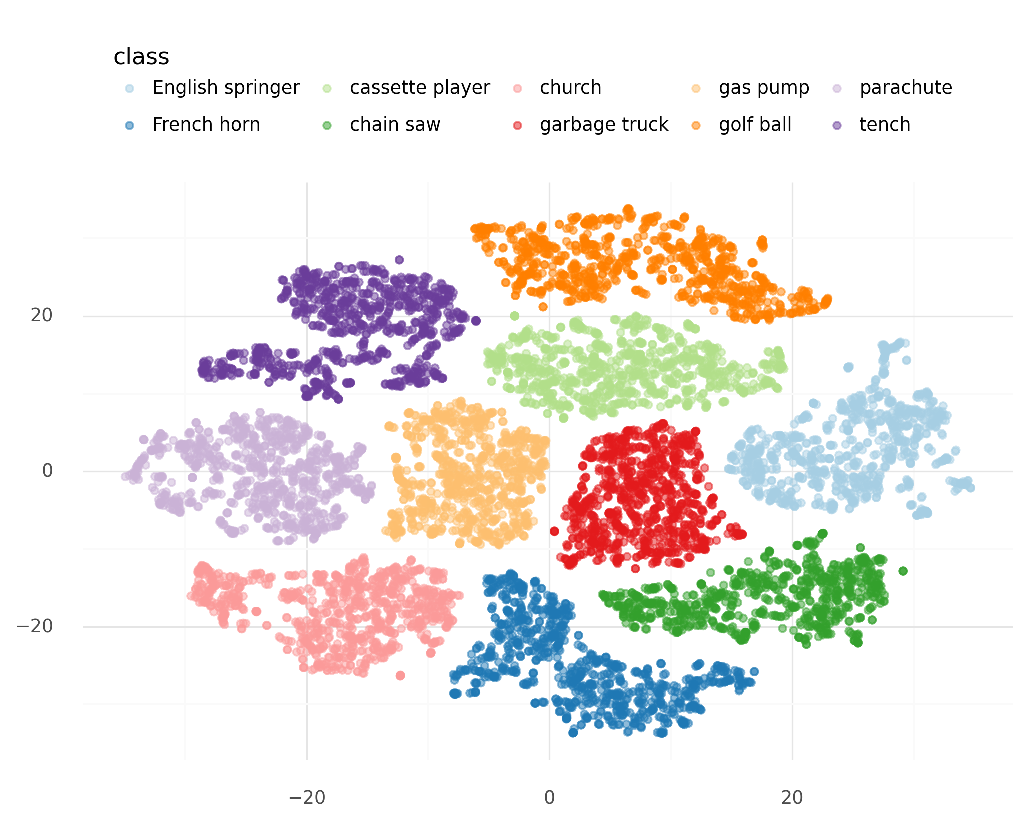
\includegraphics[width=.65\linewidth]{figure/somefig1.pdf}
\caption{Yes, put a few words or sentences here explaining what is in the figure.}
\label{fig:somefig1}
\end{figure}

Figure \ref{fig:someotherfigs} presents some summaries of the performance of our model.
The left panel of Figure \ref{fig:someotherfigs} presents something.
The right panel of Figure \ref{fig:someotherfigs} presents some other things.

\begin{figure}[htbp]
\begin{minipage}{0.53\linewidth}
  \centering
  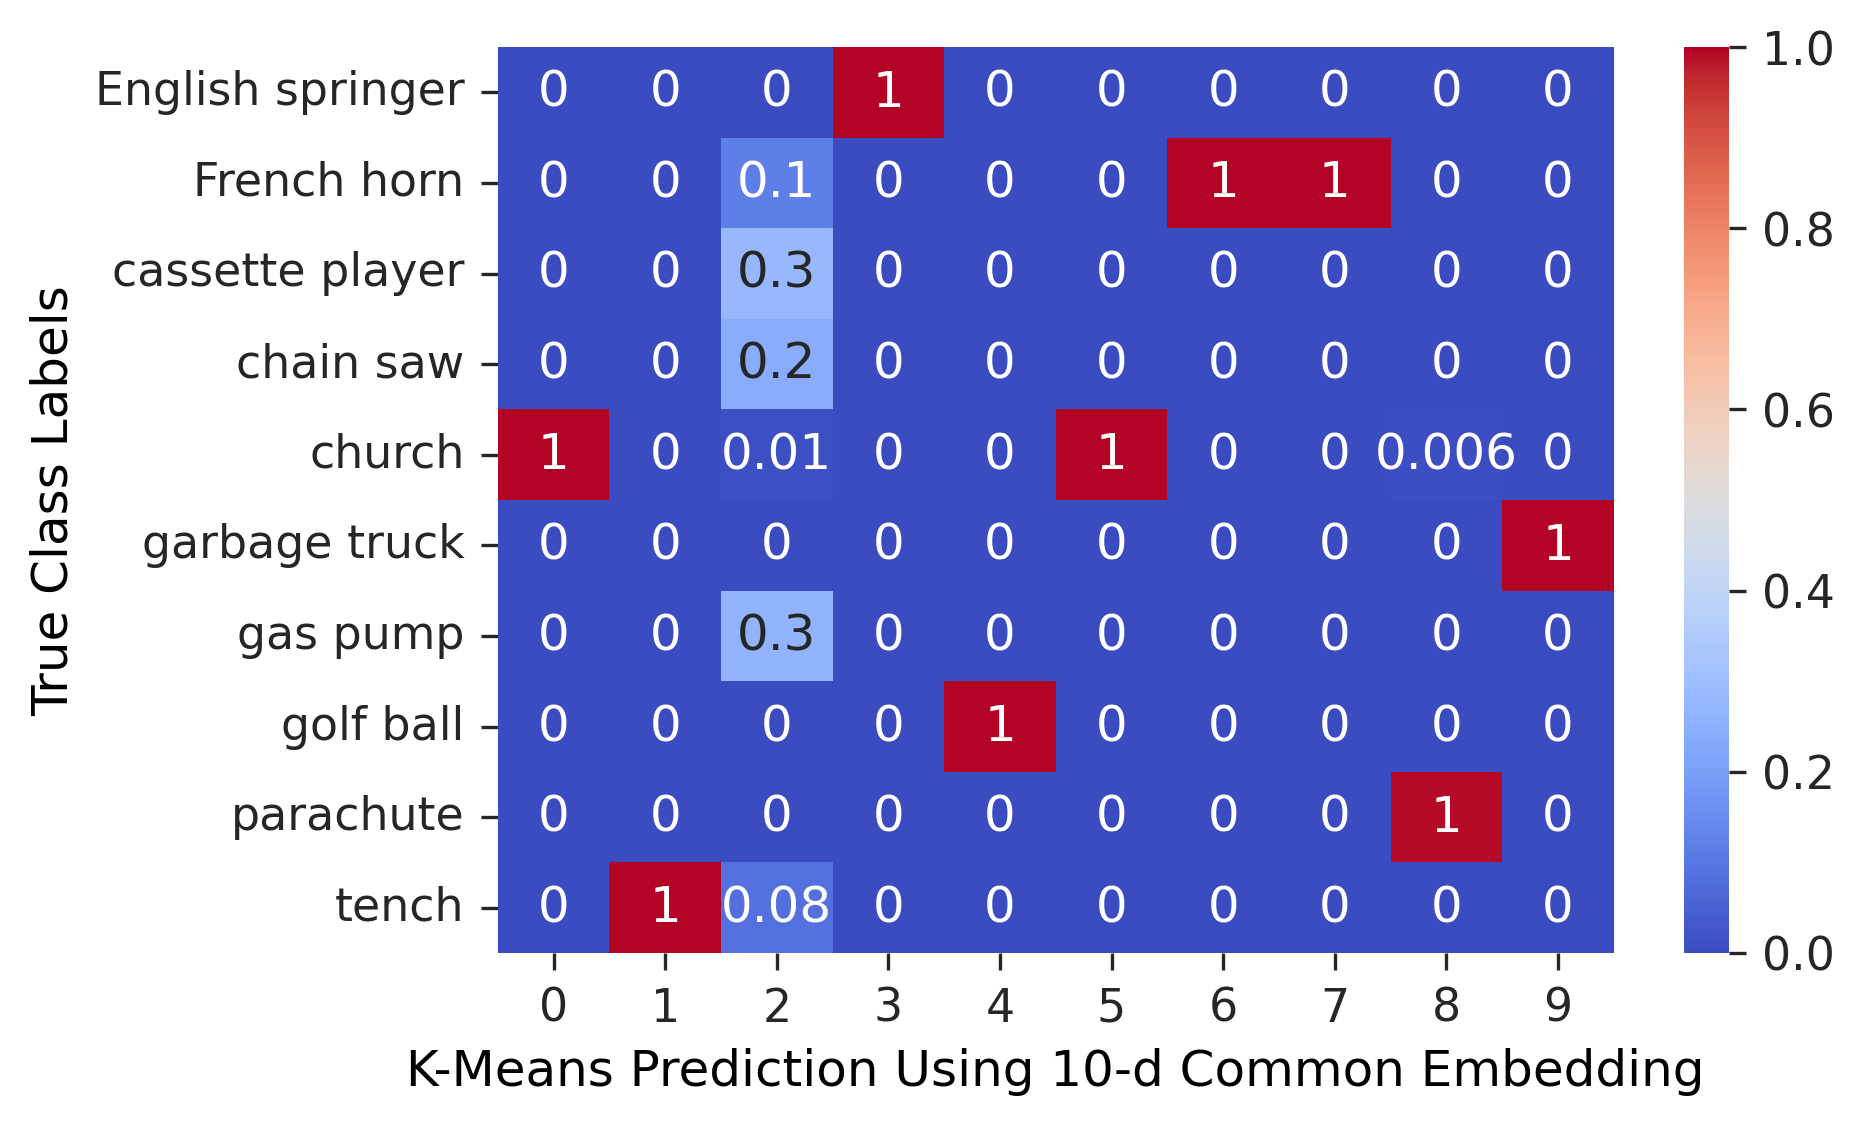
\includegraphics[width=\linewidth]{figure/somefig2.png}
\end{minipage}
\begin{minipage}{0.42\linewidth}
  \centering
  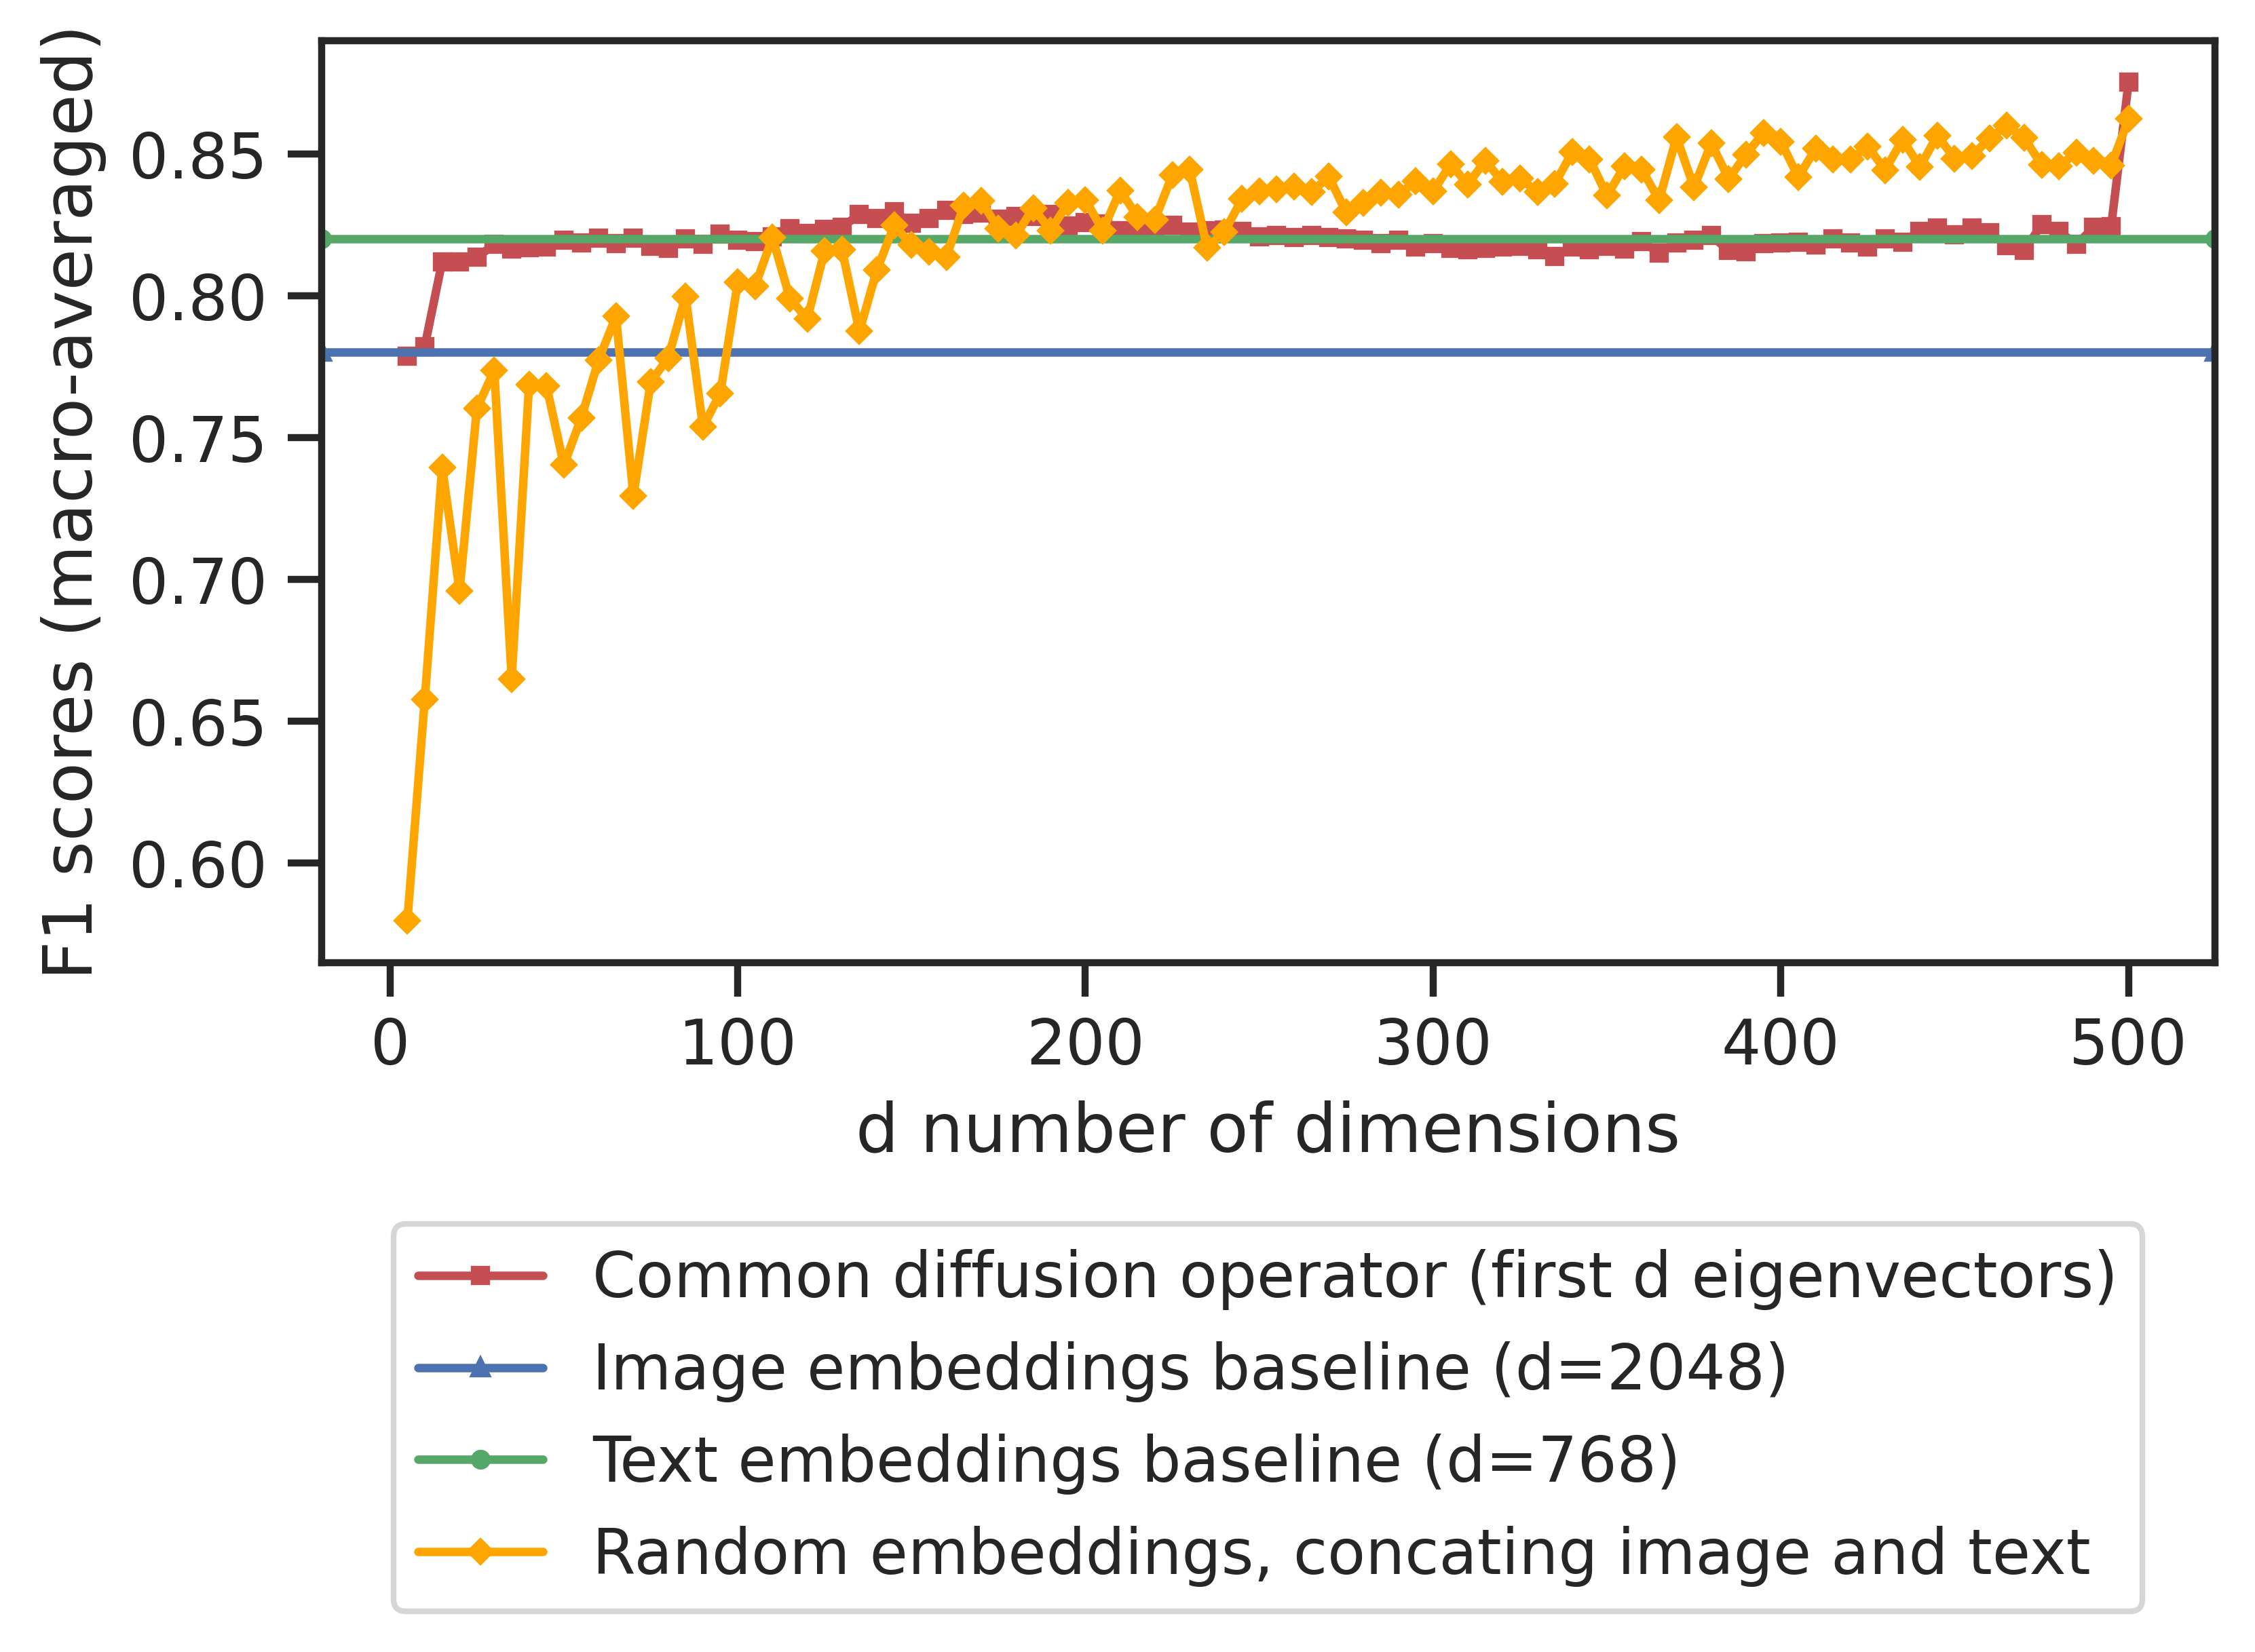
\includegraphics[width=\linewidth]{figure/somefig3.png}
\end{minipage}
\caption{You can put figures side-by-side as well.}
\label{fig:someotherfigs}
\end{figure}


\subsection{Table Examples}

Table \ref{tab:sometab1} presents some summary of the data.

\begin{table}[htbp]
\caption{Some Table Caption}
\label{tab:sometab1}
\resizebox{0.4\linewidth}{!}{\centering
\begin{tabular}{lll}
\toprule
\multicolumn{2}{c}{Part}                   \\
\cmidrule(r){1-2}
Name     & Description     & Size ($\mu$m) \\
\midrule
Dendrite & Input terminal  & $\sim$100     \\
Axon     & Output terminal & $\sim$10      \\
Soma     & Cell body       & up to $10^6$  \\
\bottomrule
\end{tabular}}
\end{table}

Table \ref{tab:sometab2} presents some summaries of the performance of our model.

\begin{table}[htbp]
\caption{Some Other Table Caption}
\label{tab:sometab2}
\resizebox{0.9\linewidth}{!}{\centering
\begin{tabular}{l|lcccccc}
\toprule
Method & Modality & Edit distance & BLEU & METEOR & Precision & Recall & F1 \\ \midrule
PDF                  & All      & 0.255 & 65.8 & 82.1 & 77.1 & 81.4 & 79.2 \\ \hline
GROBID               & All      & 0.312 & 55.6 & 71.9 & 74.0 & 72.1 & 73.0 \\ \cline{2-8}
                     &Tables    & 0.626 & 25.1 & 64.5 & 61.4 & 80.7 & 69.7 \\
+ LaTeX OCR %
                     & Plain text &0.363 & 57.4 & 69.2 & 82.1 & 70.5 & 75.9 \\
                     & Math     & 0.727 & 0.3 & 5.0 & 11.0 & 8.6 & 9.7 \\ \hline
\multirow{4}{*}{Nougat base (350M$^\ast$)} & All & \bf 0.071 & \bf 89.1 & \bf 93.0 & 93.5 & \bf 92.8 & \bf 93.1 \\ \cline{2-8}
                     & Tables     & 0.211 & 69.7 & 79.1 & 75.4 & 80.7 & 78.0 \\ 
                     & Plain text & 0.058         & 91.2 & 94.6   & 96.2      & 95.3   & 95.7 \\
                     & Math       & 0.128         & 56.9 & 75.4   & 76.5      & 76.6   & 76.5 \\ \bottomrule
\end{tabular}}
\end{table}

\subsection{Equations and Algorithms Examples}

Algorithm \ref{alg:fuzzyKmeans} implements Fuzzy K-means.

\begin{algorithm}
\caption{Fuzzy K-means clustering algorithm}
\label{alg:fuzzyKmeans}
\begin{enumerate}
    \item Choose primary centroids $v_{k}$
    \item Compute the membership degree of all feature vectors in all clusters
    \begin{equation}
    u_{ki}  = \frac{1}{ \sum_{j=1}^K ( \frac{D^{2}(x_{i} - v_{k})}{D^{2}(x_{i} - v_{j})})^\frac{2} 
    {m-1}}
    \label{eq:kmeans}
    \end{equation}
\end{enumerate}
\end{algorithm}

Algorithm \ref{alg:net} calculates net activation.


\begin{algorithm}
\caption{Computing Net Activation}
\label{alg:net}
% \DontPrintSemicolon
% \LinesNumbered
\KwIn{$x_1, \ldots, x_n, w_1, \ldots, w_n$}
\KwOut{$y$, the net activation}
$y\leftarrow 0$\;
\For{$i\leftarrow 1$ \KwTo $n$}{
$y \leftarrow y + w_i*x_i$\;
}
\end{algorithm}

In Variational Autoencoder (VAE), we directly maximize the Evidence Lower Bound (ELBO) using the following Equations \ref{eq:bla}--\ref{eq:blablabla}.
\begin{align}
  \mathbb{E}_{q_{\boldsymbol{\phi}}(\boldsymbol{z}\mid\boldsymbol{x})}\left[\log\frac{p(\boldsymbol{x}, \boldsymbol{z})}{q_{\boldsymbol{\phi}}(\boldsymbol{z}\mid\boldsymbol{x})}\right]
  &= \mathbb{E}_{q_{\boldsymbol{\phi}}(\boldsymbol{z}\mid\boldsymbol{x})}\left[\log\frac{p_{\boldsymbol{\theta}}(\boldsymbol{x}\mid\boldsymbol{z})p(\boldsymbol{z})}{q_{\boldsymbol{\phi}}(\boldsymbol{z}\mid\boldsymbol{x})}\right] \label{eq:bla} \\
  &= \mathbb{E}_{q_{\boldsymbol{\phi}}(\boldsymbol{z}\mid\boldsymbol{x})}\left[\log p_{\boldsymbol{\theta}}(\boldsymbol{x}\mid\boldsymbol{z})\right] + \mathbb{E}_{q_{\boldsymbol{\phi}}(\boldsymbol{z}\mid\boldsymbol{x})}\left[\log\frac{p(\boldsymbol{z})}{q_{\boldsymbol{\phi}}(\boldsymbol{z}\mid\boldsymbol{x})}\right] \label{eq:blabla} \\
  &= \underbrace{\mathbb{E}_{q_{\boldsymbol{\phi}}(\boldsymbol{z}\mid\boldsymbol{x})}\left[\log p_{\boldsymbol{\theta}}(\boldsymbol{x}\mid\boldsymbol{z})\right]}_\text{reconstruction term} - \underbrace{\mathcal{D}_{\text{KL}}(q_{\boldsymbol{\phi}}(\boldsymbol{z}\mid\boldsymbol{x}) \mid\mid p(\boldsymbol{z}))}_\text{prior matching term} \label{eq:blablabla}
\end{align}

\subsection{Inline Citation Examples}

Citation in text (no parentheses): use \texttt{{\textbackslash}cite\{citekey\}}. 
For example, \cite{breiman2011}, \cite{devlin2019bert}.

Citation in parentheses: use \texttt{{\textbackslash}citep\{citekey\}}. 
For example: \citep{vaswani2023attention}, \citep{karras2019stylebased}.

% COMMENT THIS BEFORE RENDERING

%%%%%%%%%%%%%%%%%%%
%%%% REFERENCES%%%%%%%
%%%%%%%%%%%%%%%%%%%
\makereference

\bibliographystyle{style/dsc180bibstyle}


\bibliography{reference}
% To edit the contents of the ``References" section, edit \texttt{reference.bib}. Many conference websites format citations in BibTeX that you can copy into \texttt{reference.bib} directly; you can also search for the paper on Google Scholar, click ``Cite", and then click ``BibTeX" (\href{https://scholar.google.com/scholar?hl=en&as_sdt=0%2C23&q=attention+is+all+you+need&btnG=#d=gs_cit&t=1700436667623&u=%2Fscholar%3Fq%3Dinfo%3A5Gohgn6QFikJ%3Ascholar.google.com%2F%26output%3Dcite%26scirp%3D0%26hl%3Den}{here}'s an example).


%%%%%%%%%%%%%%%%%%%%%%%%%%%%%%%%%%%%%%%%%%%%%%%%%%%%%%%%
%%%% Appendix
%%%%%%%%%%%%%%%%%%%%%%%%%%%%%%%%%%%%%%%%%%%%%%%%%%%%%%%%

\clearpage
\makeappendix

\subsection{Project Proposal}


% Comment out when fixed
% !TEX TS-program = xelatex
% !BIB TS-program = bibtex
\documentclass[12pt,letterpaper]{article}
\usepackage{style/dsc180reportstyle} % import dsc180reportstyle.sty

%%%%%%%%%%%%%%%%%%%%%%%%%%%%%%%%%%%%%%%%%%%%%%%%%%%%%%%%
%%%% Title and Authors
%%%%%%%%%%%%%%%%%%%%%%%%%%%%%%%%%%%%%%%%%%%%%%%%%%%%%%%%

\title{DSC Quarter 2 Capstone Project Proposal}

\author{Bradley Nathanson \\
  {\tt bnathanson@ucsd.edu} \\\And
  Christopher Lum \\
  {\tt cslum@ucsd.edu} \\\And
  Trey Scheid \\
  {\tt tscheid@ucsd.edu} \\\And
  Tyler Kurpanek \\
  {\tt tkurpane@ucsd.edu} \\\And
  Yu-Xiang Wang \\
  {\tt yuxiangw@ucsd.edu} \\}

\begin{document}
\maketitle





\section{Proposal}
\subsection{Problem Statement}

Telemetry data is important to privatize as it encodes personally identifiable information which could be used to discover sensitive information. This data is collected from various IT devices, from satellites to personal computers. For our project, the telemetry data includes hardware and software performance metrics, monitoring, and errors. 

We will privatize 22 analysis tasks for the Intel telemetry dataset, ensuring a reasonable privacy budget (). We will implement mechanisms that balance data utility and privacy, ensuring sensitive information is protected, and allocate a reasonable privacy budget (), a parameter that governs the trade-off between accuracy and privacy.

One example of a task is to predict CPU failure. This would require a privatized logistic regression model that predicts the probability of a failure from 0-1. The model would analyze data such as CPU temperature, usage patterns, error logs, or other performance indicators. If non-privatized, this model could expose this data, as a malicious individual could do a reconstruction attack, a method to reconstruct the training data by repeatedly querying the model with various synthetic inputs. The attacker could query this model with different sets of CPU-related inputs, and, over time, the attacker could gain information such as the CPU temperature threshold for an error to occur, or whether certain system configurations have a distinct failure pattern.

\subsection{Methods}
Our methodology for privatizing the 22 telemetry analysis tasks will employ multiple privacy mechanisms, such as the exponential mechanism and the Laplace mechanism, with AutoDP serving as our core privacy accounting tool. For each analysis task, we will first evaluate the sensitivity of the computation and determine the optimal privacy mechanism to maintain utility while satisfying privacy requirements. The implementation process requires careful privacy budget allocation across multiple components of each analysis to ensure the total privacy loss remains within acceptable bounds.

The evaluation of each privatized implementation will involve a comprehensive comparison with non-private baselines to document the privacy-utility tradeoff. This includes analyzing performance metrics before and after applying privacy mechanisms, measuring accuracy degradation at various privacy budget levels, and considering computational efficiency challenges specific to telemetry data analysis. AutoDP will help quantify the privacy guarantees and guide the noise calibration process throughout implementation. 

Each privatized task will be thoroughly documented with implementation details, privacy guarantees, and performance metrics. This documentation will include privacy budget allocation strategies, noise mechanism selection rationale, and practical guidelines for future implementations. The goal is to create a comprehensive resource demonstrating how different privacy mechanisms can be effectively applied to various telemetry analysis scenarios while maintaining practical utility and ensuring strong privacy protections.


\subsection{Deliverable}
The privatized analysis tasks will be stored and shared in a public repository, (without release of source data from Intel). This is our primary contribution, to offer tools in a privatized manner. In collaboration with the accessible programs, we will publish a website that will serve to educate our peers on differential privacy. The variety of analysis tasks done in the telemetry domain can be generalized and applied to many types of data; therefore, descriptions of privacy algorithms, their motivations, and limitations can teach practitioners new methods for their own tasks. 

The Intel data as mentioned is not public (due to the customer privacy and proprietary nature). Therefore our data processing, tasks, and report will include only some metrics of performance and data quality (size, distribution, features, etc). For the information we can share, we will compare the performance of the task with that of the non-private baseline. This gives analysts a sense of the utility-privacy tradeoff in each application. 

\subsection{Impact}
By implementing differential privacy across telemetry we will create a significant impact by maintaining data confidentiality. This project will establish novel approaches to common tasks enabling hardware manufacturers to analyze system performance data while preserving strong privacy guarantees. This advances the field by demonstrating how to maintain data utility while protecting sensitive information in real-world applications. 

The research contribution includes documenting privacy-utility trade-offs and establishing guidelines for privacy budget allocation across multiple analysis tasks. Our work will demonstrate practical privacy considerations in telemetry analysis while protecting users’ participation in datasets. The methodologies developed can be adapted by other researchers working with sensitive telemetry data. 

\subsection{Success Criteria}
The success of this project is dependent on a few factors. The first two are team collaboration and schedule adherence. There are many tasks that can be privatized and there may be unique challenges for each (hence the value in sharing these!). With one-quarter complete with group work on our privatized logistic regression paper, our group is confident in our communication, task management, and problem-solving abilities. Paired with our mentor Yu-Xiang Wang, an expert in the field of differential privacy, and a seasoned professor, we are equipped to find innovative and theoretically founded methods for privatizing data tasks.

The other requirements for this project rely on data access and task availability. The Intel data is proprietary, and we have signed agreements to use the data for research, however strict access and usage terms have not been given to us yet. Previous students have worked with the contact/program at Intel successfully and we are reassured by them that we will have a usable telemetry dataset by the start of the quarter.  Similarly, there is a set of non-privatized tasks completed on this dataset by previous data scientists, their work is the foundation which we will build off of to show utility is possible even with privacy. These projects were successful implementations on the specific dataset we will have access to, this pairing therefore will continue to bear fruit as we privatize the tasks and compare baselines. 

Lastly, although we have not reviewed the dataset and tasks yet (no access), the intel program is sharing genuine telemetry information from devices with given consent as part of their program. Additionally, this HDSI-Intel partnership has been cooperating since 2020 and HDSI has used hundreds of terabytes of information. 





\end{document}
% Comment out when fixed


\subsection{Appendix A: Additional Results}
example

\subsection{Appendix B: Training Details}
example

\subsection{Appendix C: Additional Figures}
example


\end{document}